\documentclass{article}

\usepackage{amsmath}
\usepackage{graphicx}
\usepackage{epstopdf}
\usepackage{booktabs}
\usepackage{siunitx}
\usepackage{caption}
\usepackage{url}
\usepackage{abstract}
%\usepackage{tikz,pgfplots} % diagrams and data plots

\captionsetup{margin=12pt,font=small,labelfont=bf}

\renewcommand{\abstractname}{}

\setlength{\absleftindent}{30mm}
\setlength{\absrightindent}{30mm}

\newcommand{\figref}[2][\figurename~]{#1\ref{#2}}
\newcommand{\tabref}[2][\tablename~]{#1\ref{#2}}
\newcommand{\secref}[2][Section~]{#1\ref{#2}}


\begin{document}
\title{A Gaussian Sample 3 ways} 
\author{Ben McMurtry}
\date{11th November 2016} 	
\maketitle





\section{Introduction}
\label{sec:introduction}

A random-number generator (RNG) is a computational or physical device designed to generate a sequence of numbers or symbols that cannot be reasonably predicted better than by a random chance\cite{RNG}.

Some methods for generating random data, have existed since ancient times, such as the ``classic'' examples of rolling dice, flipping coins  or  shuffling a pack of cards.

A program was written to investigate the speed and randomness of four different Random Number Generators, one RNG using the POSIX function ``random()'' which is designed to give random variates with a uniform probability density between the lower and upper limit parameters given, and then three RNGs (The Approximate Method, The Box-Muller Method, and The Rejection Method) which take uniform random numbers (given by the first RNG), and give out random variates with a Normal probability density. 

The output variates of these RNGs were then converted to the required Gaussian with mean 5.0 and variance 2.0 by multiplying them by $\sqrt{variance}$ and then adding the mean.





\section{RNG}

The first RNG method in the program uses the ``random()'' function, which comes with the standard library on POSIX systems. It is described as a (non)linear additive feedback random number generator employing a default table of size 31 long integers to return successive pseudo-random numbers in the range from 0 to RANDOM\_MAX\cite{Random}.  This function has a very large period of approximately 16 * (($2^{31}$) - 1). The number returned by ``random()'' is then divided by RANDOM\_MAX , and then multiplied by a defined range (UPPER - LOWER) and added to the lower bound of the range (LOWER), meaning it is now creating a random variate, with uniform probability density, between the bounds UPPER and LOWER. 





\section{Approximate Method}

The Approximate Method is a simple algorithm for generating random variates with a normal distribution. The method uses the Central Limit Theorem, which states that, for most scenarios when independent random variables are added, their sum tends toward a normal distribution\cite{Central}.

The algorithm used in the code to generate random variates from this method is as follows:

\begin{equation}
Z = (\sum_{j=1}^{12}{U_j}) - 6 
\end{equation}

Where $U_j$ are independently and identically distributed random variates between 0 and 1 (made with RNG).





\section{Box-Muller Method}

The Box-Muller transform, discovered in 1958, generates pairs of independent, standard, normally distributed (zero expectation, unit variance) random numbers, given a source of uniformly distributed random numbers\cite{Box-Muller}.

The algorithm used to generate random variates from this method is as follows:

\begin{enumerate}
\item 
Generate $U_1$ and $U_2$ as independent U[0,1] random variables (made with RNG)
\item 
$z_{0}=\sqrt{-2\ln U_{1}}\cos(2\pi U_{2}) = Rcos(\Theta)$

$z_{1}=\sqrt{-2\ln U_{1}}\sin(2\pi U_{2}) = Rsin(\Theta)$
\end{enumerate} 

The derivation is based on a property of a two-dimensional Cartesian system, where X and Y coordinates are described by two independent and normally distributed random variables, and can be understood by seeing that:

$x_1	= e^{\frac{-(z_1^2+z_2^2)}{2}}$

$x_2	= \frac{1}{2\pi}tan^{-1}(\frac{z_2}{z_1})$

which, taking the Jacobian yields:

$f(z_1, z_2) = -[\frac{1}{\sqrt{2\pi}}e^{\frac{-z_1^2}{2}}]  [\frac{1}{\sqrt{2\pi}}e^{\frac{-z_2^2}{2}}]$





\section{Rejection Method}

In mathematics, rejection sampling (also commonly called the acceptance-rejection method or ``accept-reject algorithm") is a type of Monte Carlo method\cite{Rejection}.

Rejection sampling is based on the observation that to sample a random variable one can perform a uniformly random sampling of the 2D cartesian graph, and keep the samples in the region under the graph of its density function. 

This is usually done by utilising a method known as the inverse transform method\cite{Inverse}.

If we want to sample from a complicated probability density function such as a normal distribution $p(x)$:

\begin{equation}
p(x) = \frac{1}{\sqrt{2\pi}} exp(-\frac{x^2}{2})
\end{equation}

which is not easy to invert. We can instead use a majorising function $a(x)$, which is larger than $p(x)$ for the range of x we are interested in:

\begin{equation}
a(x) = \frac{0.50}{1+x^2} = 0.50\frac{d}{dx}arctan(x)
\end{equation}

This function can then be normalised by dividing it by its integral from -$\infty$ to $\infty$. And then integrated from -$\infty$ to $x$ to give its Cumulative Density Function, which is then inverted, and passed U[0,1] variates (made with RNG) to create the random variates $Y$, 

The algorithm used to generate random variates from this method is then as follows:

\begin{enumerate}
\item Generate random variate $Y$ having density $R(Y)$.
\item Generate U from U[0,1] (independent of $Y$ in step 1!)
\item If $U \leq \frac{f(y)}{a(y)}$ then return $X = Y$, convert to gaussian variate, and exit (accept)
\item Else, go to Step 1 (reject)
\end{enumerate}





\section{Discussion}

The RNGs described above were all written into the program, a sample of random variates from each created, and the time taken to do so printed to standard out. The samples were then investigated by another function which calculates their minimum, maximum, mean, standard deviation, and standard error, and plots them as a normalised histogram alongside the probability density function they are supposed to obey. The output for each, at a sample size of 10,000 and 1,000,000 is discussed below. It should be noted that the program creates an array of doubles with the designated size of the sample, so exceeding 1,000,000 variates can lead the program to exit, due to the large required RAM for the array.

For the RNG function with random(), the function was given a lower bound of 3.0 and an upper bound of 7.0. For the Gaussian distributions, they have all been designed such that their mean should be 5.0 and their variance should be 2.0 (therefore standard deviation = $\sqrt{2}$ = 1.41421).





\subsection{RNG}

From the programs results in Figures 1 and 2, we can see that the RNG function does a reasonably good job of producing a uniform distribution, very quickly (1 million variates in 0.0098s). With a sample of 1million, it is very hard to detect much deviation from the square distribution, as is shown by the very accurate mean of 4.99997, and the very low standard error of 0.0014. It is, however, possible to see some deviation and possibly even some periodicity in the plot with only 10,000 datapoints.

From this data we can conclude that we can, with reasonable safety, use this function to produce the random U[0,1] variates required for the following three RNGs, especially in the case of using high numbers of variates $>$10,000.

\begin{figure}[htb]
\centering{
\includegraphics[width=70mm]{RNG4.png}
\caption{RNG method: Time = 9e-05s. N = 10,000. Min = 3.00003. Max = 6.99981. Mean = 5.01147. Std\_dev = 1.15306. Std\_error = 0.0115306.}
\label{RNG4}
}
\end{figure}

\begin{figure}[htb]
\centering{
\includegraphics[width=70mm]{RNG6.png}
\caption{RNG method: Time =  0.009752s. N = 1,000,000. Min = 3.00001. Max = 7. Mean = 4.99997. Std\_dev = 1.15448. Std\_error = 0.00115448.}
\label{RNG6}
}
\end{figure}





\subsection{Approximate Method}

From the programs results in Figures 3 and 4, we can see the Approximate method creates a close approximation to the desired Gaussian distribution. This is concluded as the 1,000,000 variate sample produces a mean with an error of $\approx0.008\%$, a standard deviation with error of $\approx0.03\%$, and a standard error of $\approx0.0014139$.

The speed of the approximate method may appear fast (0.13s for 1,000,000 variates), but it is in fact relatively slow compared to some other methods due to the fact that it has to produce 12 random [0,1] variates to produce just one random gaussian variate. It is however still faster than the rejection method.

\begin{figure}[htb]
\centering{
\includegraphics[width=70mm]{Approx4.png}
\caption{Approximate method: Time =  0.001541s. N = 10,000. Min = 0.329878. Max = 10.2426. Mean = 5.00218. Std\_dev = 1.40877. Std\_error = 0.0140877.}
\label{Approx4}
}
\end{figure}

\begin{figure}[htb]
\centering{
\includegraphics[width=70mm]{Approx6.png}
\caption{Approximate method: Time =  0.129368s. N = 1,000,000. Min = -1.24908. Max = 11.0898. Mean = 5.00042. Std\_dev = 1.4139. Std\_error = 0.0014139}
\label{Approx6}
}
\end{figure}





\subsection{Box-Muller Method}

From the programs results in Figures 5 and 6, we can see that the Box-Muller method creates a fairly close approximation to the desired Gaussian distribution. This is based on the fact that the 1,000,000 variate sample produces a mean with an error of $\approx0.04\%$, a standard deviation with error of $\approx0.05\%$, and a standard error of $\approx0.0014136$.

This method is easily the fastest of the three (0.045s for 1,000,000 variates), and it is easy to see why, as it only needs one random [0,1] variate per random gaussian variate produced, and only has to do N/2 caclulations if the code takes advantage of complex.h and its ability to compute cosine and sine simultaneously.

\begin{figure}[htb]
\centering{
\includegraphics[width=70mm]{BoxM4.png}
\caption{Box-Muller method: Time =  0.000432s. N = 10,000. Min = -0.215672. Max = 10.4329. Mean = 5.01513. Std\_dev = 1.41768. Std\_error = 0.0141768}
\label{BoxM4}
}
\end{figure}

\begin{figure}[htb]
\centering{
\includegraphics[width=70mm]{BoxM6.png}
\caption{Box-Muller method: Time =  0.04548s. N = 1,000,000. Min = -2.16552. Max = 11.8082. Mean = 5.00196. Std\_dev = 1.4136. Std\_error = 0.0014136}
\label{BoxM6}
}
\end{figure}





\subsection{Rejection Method}

From the programs results in Figures 7 and 8, we can see that the Rejection method creates a very close approximation to the desired Gaussian distribution. This is concluded as the 1,000,000 variate sample produces a mean with an error of $\approx0.003\%$, a standard deviation with error of $\approx0.02\%$, and a standard error of $\approx0.0014145$.

The rejection method is, however, the slowest, when compared to the other two methods (0.302s for 1,000,000 variates) explained by the fact that the method has to produce an extra random [0,1] variate each time the reject step is reached for each random gaussian variate. The number of times this occurs should be based on the closeness of the majorising function to the desired function, which can be seen in \figref{majorising}.

\begin{figure}[htb]
\centering{
\includegraphics[width=70mm]{Reject4.png}
\caption{Rejection method: Time =  0.003493s. N = 10,000. Min = -0.432916. Max = 10.5475. Mean = 4.99807. Std\_dev = 1.40977. Std\_error = 0.0140977}
\label{Reject4}
}
\end{figure}

\begin{figure}[htb]
\centering{
\includegraphics[width=70mm]{Reject6.png}
\caption{Rejection method: Time =  0.302239s. N = 1,000,000. Min = -1.85767. Max = 11.5288. Mean = 5.00015. Std\_dev = 1.4145. Std\_error = 0.0014145}
\label{Reject6}
}
\end{figure}

Doing some analysis, by integrating $p(x)$ and $a(x)$ between -3 to 3, we find that $p(x)$ is $\approx$ $\frac{4}{5}$ times as big as $a(x)$. This would imply that the reject step is reached only 1 in 5 times.

The time taken for this method, however, is longer than the approximate method, which might seem to imply that over 12 rejections per variate, on average, however, the time of this method is more likely high due to the required logic steps of comparing the size $p(y)$ and $a(y)$.

\begin{figure}[htb]
\centering{
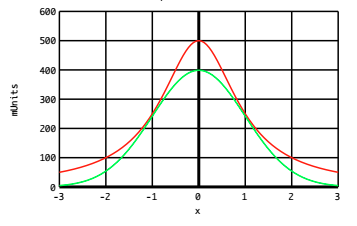
\includegraphics[width=80mm]{majorising.png}
\caption{The normal distribution in green, and the majorising function $a(x)$ used in red.}
\label{majorising}
}
\end{figure}





\section{Conclusions}

This program can investigate the properties of one uniform RNG, and three Gaussian RNGs and determine which of them returns a sample of certain size quickest, and how close to the desired probability density function the sample of variates turns out. Additionally it can plot the data as a histogram so that one could determine by eye how well they fit the theoretical probability density function.

With a sample size of 1,000,000, all three RNGs do a very good job of creating gaussian variates, which by eye fit the gaussian curve very well. Going down to a sample size of 10,000, the RNGs do not create such a perfect gaussian histogram, although none are clearly worse than the others at this size, and the noise could possibly be due to the random [0,1] variate noise seen in Figure 1, rather than any issue with the Gaussian variate generating methods.

The Rejection method appears to create the most accurate sample, but is the slowest method, whilst the Box-Muller method appears to be the fastest, with the least accurate sample. The Approximate method, lying in the middle on both scales.

If one wanted to expand the scope of the project and to have more conclusive evidence for the fidelity of the randomness of the data produced, one could perform, for instance Pearson's Chi-Squared Test on the data, which gives some quantitative measure of the likelihood that any fluctuations in the data occurred by chance\cite{Test}.

One could also test the samples a number of times and average the time taken, or even test the RNGs for different seeds of srandom() (which for the results in this report was left at it's default of srandom(1)), to do this, simply uncomment line 211 of the code, to have the seed dynamically allocated by time.h.





\begin{thebibliography}{9}
\bibitem{RNG}
\url{https://en.wikipedia.org/wiki/Random_number_generation#.22True.22_vs._pseudo-random_numbers}
\bibitem{Random}
\url{http://www.mathstat.dal.ca/~selinger/random/}
\bibitem{Central}
\url{https://en.wikipedia.org/wiki/Central_limit_theorem}
\bibitem{Box-Muller}
\url{http://projecteuclid.org/DPubS/Repository/1.0/Disseminate?view=body&id=pdf_1&handle=euclid.aoms/1177706645}
\bibitem{Rejection}
\url{https://en.wikipedia.org/wiki/Rejection_sampling}
\bibitem{Inverse}
\url{https://en.wikipedia.org/wiki/Inverse_transform_sampling}
\bibitem{Test}
\url{https://en.wikipedia.org/wiki/Pearson's_chi-squared_test}

\end{thebibliography}





\end{document}
